\section{投影子缀加波(Projector Augmented Wave, PAW)方法}
PAW方法是\textrm{Bl\"ochl}于1994年独立提出来的一种计算方法\cite{PRB50-17953_1994},该方法的基本思想与OPW很相似,但同时结合了赝势方法和APW方法的优点,达到平衡计算效率和精度的目的。PAW方法刚提出来的时候并未引起注意,直到1999年\textrm{Kresse}指明了PAW方法和USPP方法的密切关联,USPP方法的计算程序只要经过简单改造就能扩展为PAW方法,有力地推动了PAW方法的广泛应用\cite{PRB59-1758_1999}。现在PAW方法已经成为最主要的可支持第一原理分子动力学(Ab initio Molecular Dynamics, AIMD)。

\subsection{PAW方法的基本思想}
与一般赝势方法不同,PAW方法的目标是全电子(all-electron)波函数\footnote{注意,“全电子”在\textrm{Bl\"ochl}原始文献\inlinecite{PRB50-17953_1994}中与“真实电子波函数”意义相近,强调电子在原子核附近的振荡行为,但并未严格区分价电子与芯电子;~而在\textrm{Kresse}的文献\inlinecite{PRB59-1758_1999}中则是明确指价电子波函数。%强调价电子波函数因与芯层电子正交而在原子核附近振荡;
此外,与“全电子”概念密切关联的是“全势(full-potential)”,两者在具体语境中有一定的区别,“全势”强调的是重现价电子感受到的势函数的效果。},体系中全部电子构成\textrm{Hilbert}空间,价电子与芯层态彼此正交,使得波函数在\textrm{Muffin-tin}球内振荡。
\textrm{Bl\"ochl}假设全电子波函数$|\Psi\rangle$与赝波函数$|\tilde\Psi\rangle$满足线性变换,即满足:
\begin{equation}
	|\Psi\rangle=\mathbf{\tau|}\tilde\Psi\rangle
	\label{eq:PAW-Blochl-01}
\end{equation}
%	$$\tau=\mathbf{1}+\sum_{\mathrm R}\hat\tau_{\mathrm R}$$
在原子核附近的$r_c$范围内\footnote{习惯上这个区域称为缀加区(\textrm{Augmentation region}).},除了平面波,还引入原子分波函数展开来表示波函数:
\begin{equation}
	|\Psi\rangle=|\tilde\Psi\rangle+\sum_i(|\phi_i\rangle-|\tilde\phi_i\rangle)\langle\tilde p_i|\tilde\Psi\rangle
	\label{eq:PAW-Blochl-02}
\end{equation}
在$r_c$外$|\tilde\Psi\rangle$与$|\Psi\rangle$变换前后保持不变,因此线性变换$\mathbf{\tau}$可表示为:
\begin{equation}
	\mathbf{\tau}=\mathbf{1}+\sum_i(|\phi_i\rangle-|\tilde\phi_i\rangle)\langle\tilde p_i|
	\label{eq:PAW-Blochl-03}
\end{equation}
其中$|\tilde p_i\rangle$是\textrm{MT}球内的投影函数,$i$表示原子位置$\vec R$、原子轨道($l,m$)和能级$\epsilon_k$的指标。\textrm{PAW}的波函数与赝波函数的关系,可以用图\ref{PAW_basic}表示。
\begin{figure}[h!]
\centering
\includegraphics[height=2.35in,width=4.1in,viewport=0 0 1280 745,clip]{PAW-baseset.png}
%\includegraphics[height=1.8in,width=4.in,viewport=30 210 570 440,clip]{PAW_projector.eps}
\caption{\small \textrm{The analysis of PAW basic function.}}%(与文献\cite{EPJB33-47_2003}图1对比)
\label{PAW_basic}
\end{figure}

\subsection{PAW表示下的能量表示与补偿电荷}
\textrm{PAW}方法通过投影算符和赝波函数实现全电子波函数计算,因此完整的\textrm{PAW}方法下,一般算符的期望值计算为
\begin{equation}
	\langle A \rangle=\langle\Psi|\mathbf{A}|\Psi\rangle=\langle\tilde\Psi|\mathbf{\tau}^{\dag}\mathbf{A}\mathbf{\tau}|\tilde\Psi\rangle=\langle\tilde\Psi|\tilde{\mathrm{A}}|\tilde\Psi\rangle
	\label{eq:PAW-Blochl-04}
\end{equation}
式中将$\mathrm{\tau}$用式\eqref{eq:PAW-Blochl-03}展开,因此赝算符$\tilde A$可表示为
\begin{equation}
	\tilde A=\mathbf{A}+\sum_i|\tilde p_i\rangle(\langle\phi_i|\mathbf{A}|\phi_i\rangle-\langle\tilde\phi_i|\mathbf{A}|\tilde\phi_i\rangle)\langle\tilde p_i|
	\label{eq:PAW-Blochl-05}
\end{equation}
%不难看出,赝重叠算符$\tilde O$可展开为
%\begin{equation}
%	\tilde O=\mathbf{1}+\sum_i|\tilde p_i\rangle(\langle\phi_i|\phi_i\rangle-\langle\tilde\phi_i|\tilde\phi_i\rangle)\langle\tilde p_i|
%	\label{eq:PAW-Blochl-06}
%\end{equation}
实空间中,电荷密度的算符为$|r\rangle\langle r|$,根据式\eqref{eq:PAW-Blochl-03},则电荷密度的计算
\begin{equation}
	n(\vec r)=\tilde n(\vec r)+n^1(\vec r)-\tilde n^1(\vec r)
	\label{eq:PAW-Blochl-07}
\end{equation}
这里
\begin{displaymath}
	\begin{aligned}
		\tilde n(\vec r)=&\sum_nf_n\langle\tilde\Psi_n|\vec r\rangle\langle\vec r|\tilde\Psi_n\rangle \\
n^1(\vec r)=&\sum_{n,(i,j)}f_n\langle\tilde\Psi_n|\tilde p_i\rangle\langle\phi_i|\vec r\rangle\langle\vec r|\phi_j\rangle\langle\tilde p_j|\tilde\Psi_n\rangle \\
\tilde n^1(\vec r)=&\sum_{n,(i,j)}f_n\langle\tilde\Psi_n|\tilde p_i\rangle\langle\tilde\phi_i|\vec r\rangle\langle\vec r|\tilde\phi_j\rangle\langle\tilde p_j|\tilde\Psi_n\rangle
	\end{aligned}
\end{displaymath}
$f_n$是占据态的电子数。注意,这里的$n^1$和$\tilde n^1$中包含了芯层电荷的贡献,即$\sum_n\langle\phi_n^c|\vec r\rangle\langle\vec r|\phi_n^c\rangle$,$\sum_n\langle\tilde\phi_n^c|\vec r\rangle\langle\vec r|\tilde\phi_n^c\rangle$和$\sum_n\langle\tilde\Psi_n^c|\vec r\rangle\langle\vec r|\tilde\Psi_n^c\rangle$。但是实际应用中,一般都是直接构造芯层态电荷密度,并不考虑芯层态波函数。

类似地,根据\textrm{DFT}理论,体系总能量泛函可以表示为
\begin{equation}
	\begin{aligned}
		E&=\sum_nf_n\langle\Psi_n|-\dfrac12\nabla^2|\Psi_n\rangle\\
		 &+\dfrac12\int\mathrm{d}\vec r\int\mathrm{d}\vec r^{\prime}\dfrac{(n+n^Z)(n+n^Z)}{|\vec r-\vec r^{\prime}|}+\int\mathrm{d}\vec r n\epsilon_{\mathrm{XC}}(n)
	\end{aligned}
	\label{eq:PAW-Blochl-08}
\end{equation}
在\textrm{PAW}框架下,总能可分解为$E=\tilde E+E^1-\tilde E^1$,每一项分别表示为:
\begin{equation}
	\begin{aligned}
		\tilde E&=\sum_nf_n\langle\tilde\Psi_n|-\dfrac12\nabla^2|\tilde\Psi_n\rangle\\
		 &+\dfrac12\int\mathrm{d}\vec r\int\mathrm{d}\vec r^{\prime}\dfrac{(\tilde n+\hat n)(\tilde n+\hat n)}{|\vec r-\vec r^{\prime}|}+\int\mathrm{d}\vec r \tilde n\bar v+\int\mathrm{d}\vec r \tilde n\epsilon_{\mathrm{XC}}(\tilde n)
 	\end{aligned}
	\label{eq:PAW-Blochl-09}
\end{equation}
\begin{equation}
	\begin{aligned}
		E^1&=\sum_{n,(i,j)}f_n\langle\tilde\Psi_n|\tilde p_i\rangle\langle\phi_i|-\dfrac12\nabla^2|\phi_j\rangle\langle\tilde p_j|\tilde\Psi_n\rangle\\
		 &+\dfrac12\int\mathrm{d}\vec r\int\mathrm{d}\vec r^{\prime}\dfrac{(n^1+n^Z)(n^1+n^Z)}{|\vec r-\vec r^{\prime}|}+\int\mathrm{d}\vec r n^1\epsilon_{\mathrm{XC}}(n^1)
 	\end{aligned}
	\label{eq:PAW-Blochl-10}
\end{equation}
\begin{equation}
	\begin{aligned}
		\tilde E^1&=\sum_{n,(i,j)}f_n\langle\tilde\Psi_n|\tilde p_i\rangle\langle\tilde\phi_i|-\dfrac12\nabla^2|\tilde\phi_j\rangle\langle\tilde p_j|\tilde\Psi_n\rangle\\
		 &+\dfrac12\int\mathrm{d}\vec r\int\mathrm{d}\vec r^{\prime}\dfrac{(\tilde n^1+\hat n)(\tilde n^1+\hat n)}{|\vec r-\vec r^{\prime}|}+\int\mathrm{d}\vec r \tilde n^1\bar v+\int\mathrm{d}\vec r \tilde n^1\epsilon_{\mathrm{XC}}(\tilde n^1)
 	\end{aligned}
	\label{eq:PAW-Blochl-11}
\end{equation}
式\eqref{eq:PAW-Blochl-09}和\eqref{eq:PAW-Blochl-11}中$\bar v$是缀加区内的任意局域函数,只要该区域内满足条件$\tilde n=\tilde n^1$,则$\bar v$对总能量的贡献为0。与赝势方法类似,$\bar v$取去屏蔽局域赝势。

类似地,式\eqref{eq:PAW-Blochl-09}和\eqref{eq:PAW-Blochl-11}中$\hat n$为补偿电荷,取值范围限于缀加区。与超软赝势中的补偿电荷的要求类似,\textrm{PAW}方法中的$\hat n$存在使得电荷密度$(n^1+n^Z)$和$(\tilde n^1+\hat n)$在缀加区外的多极矩贡献相等,因此不必再考虑电荷在缀加区外的相互作用,只需考虑$\hat n$在$\tilde E$中的贡献。$\hat n$可表示为单个原子截断区间的补偿电荷之和,即$\hat n=\sum_R\hat n_R$,并且$\hat n_R(r)$可用\textrm{Gaussian}函数展开,即
\begin{equation}
	\hat n_R(r)=\sum_{L=(l,m)}g_{RL}(r)Q_{RL}
	\label{eq:PAW-Blochl-12}
\end{equation}
式中$g_{RL}(r)$是广义的\textrm{Gaussian}函数,表示如下
	$$g_{RL}(r)=C_l|r-R|^lY_L(r-R)\mathrm{e}^{-(|r-R|/r_c)^2}$$
其系数$C_l$是归一化系数,由条件
	$\int\mathrm{d}rr^lY_L(r)g_L(r)=1$
确定。
式\eqref{eq:PAW-Blochl-12}的$Q_{RL}$由构造补偿电荷所须满足的多极矩条件确定
	$$Q_{RL}=\int\mathrm{d}r|r-R|^l\big[n_R^1(r)+n_R^Z(r)-\tilde n_R^1(r)\big]Y_L^{\ast}(r-R)$$

一般来说,原子的补偿电荷的\textrm{Gaussian}展开在缀加区会快速衰减,这意味着最终需要很高的平面波来展开。在\textrm{Bl\"ochl}的方案中,建议引入新的补偿电荷$\hat n^{\prime}$,满足条件:~\footnote{这是\textrm{Bl\"ochl}方案与后来\textrm{Kresse}方案处理补偿电荷的主要区别。}
	\begin{itemize}
		\item $\hat n^{\prime}$与$\hat n$具有相同的多极矩(保留原来的补偿电荷的基本要求)
		\item $\hat n^{\prime}$的\textrm{Gaussian}函数展开的衰减半径$r_c^{\prime}$比$r_c$大得多,可以用很少的平面波展开
	\end{itemize}
因此,能量$\tilde E$中的静电相互作用可以表示为
	\begin{equation}
		\begin{aligned}
			&\dfrac12\int\mathrm{d}r\int\mathrm{d}r^{\prime}\dfrac{(\tilde n+\hat n)(\tilde n+\hat n)}{|r-r^{\prime}|}\\
			=&\underline{\dfrac12\int\mathrm{d}r\int\mathrm{d}r^{\prime}\dfrac{(\tilde n+\hat n^{\prime})(\tilde n+\hat n^{\prime})}{|r-r^{\prime}|}}
			+\underline{\int\mathrm{d}r\tilde n(r)\hat v(r)}+\underline{\sum_{R,R^{\prime}}U_{R,R^{\prime}}}
		\end{aligned}
		\label{eq:PAW-Blochl-13}
	\end{equation}
其中第一项是平滑函数,可以在\textrm{Fourier}空间计算
	$$2\pi V\sum_G\dfrac{|\tilde n(G)+\hat n^{\prime}(G)|^2}{G^2}$$
第二项的$\hat v(r)$表示为
	$$\hat v(r)=\int\mathrm{d}r^{\prime}\dfrac{\hat n(r^{\prime})-\hat n^{\prime}(r^{\prime})}{|r-r^{\prime}|}$$
虽然$\hat v(r)$和$n(r)$一样有高\textrm{Fourier}截断,但因为$\tilde n(G)$只需要少量平面波展开,所以$\hat v(r)$的高阶部分不会对$\int\mathrm{d}r\tilde n(r)\hat v(r)$有贡献。最后一项中$U_{R,R^{\prime}}$是原子间的短程成对势
	$$U_{R,R^{\prime}}=\dfrac12\int\mathrm{d}r\int\mathrm{d}r^{\prime}\dfrac{\hat n_R(r)\hat n_{R^{\prime}}(r^{\prime})-\hat n_R^{\prime}(r)\hat n_{R^{\prime}}^{\prime}(r^{\prime})}{|r-r^{\prime}|}$$
这一项可以通过\textrm{Ewald}求和方法计算。

\subsection{PAW方法的Kohn-Sham方程与原子分波、投影函数}
在\textrm{DFT}框架下,应用\textrm{PAW}方法,除了总能量的表示外,还要考虑\textrm{Kohn-Sham}方程。根据式\eqref{eq:PAW-Blochl-05},平面波基表示的重叠算符可以写成:
\begin{equation}
	\tilde O=\mathbf{1}+\sum_{i,j}|\tilde p_i\rangle\bigg[\langle\phi_i|\phi_j\rangle-\langle\tilde\phi_i|\tilde\phi_j\rangle\bigg]\langle\tilde p_j|
	\label{eq:PAW-Blochl-14}
\end{equation}
类似地,可以得到根据定义,经典的\textrm{DFT}中\textrm{Hamilitonian}算符:%\cite{PRB50-17953_1994}
\begin{equation}
	\begin{aligned}
		\dfrac{\mathrm{d}E}{\mathrm{d}\rho}=&\dfrac{\partial\mathrm{Tr}[-\frac12\nabla^2\rho]}{\partial\rho}+\int\mathrm{d}r\dfrac{\partial E}{\partial n(r)}\dfrac{\mathrm{Tr}[|r\rangle\langle r|\rho]}{\partial\rho}\\
		=&-\dfrac12\nabla^2+v
	\end{aligned}
	\label{eq:PAW-DFT-H}
\end{equation}
这里$v(r)=|r\rangle\dfrac{\partial E}{\partial n(r)}\langle r|$。\textrm{PAW}方法中,\textrm{Hamiltonian}算符是总能量对赝电荷密度$\tilde\rho=\sum\limits_i|\tilde\Psi_n\rangle f_n\langle\tilde\Psi_n|$的变分(约束条件是$\langle\tilde\Psi_n|\tilde O|\tilde\Psi_m\rangle=\delta_{nm}$):
\begin{equation}
	\begin{aligned}
		\dfrac{\mathrm{d}E}{\mathrm{d}v\tilde\rho}=&\dfrac{\partial\mathrm{Tr}[-\frac12\nabla^2\rho]}{\partial\rho}+\int\mathrm{d}r\dfrac{\partial E}{\partial n(r)}\dfrac{\mathrm{Tr}[|r\rangle\langle r|\rho]}{\partial\rho}\\
		=&-\dfrac12\nabla^2+v
	\end{aligned}
	\label{eq:PAW-Blochl-H}
\end{equation}
注意,这里势能是$\tilde n$、$\tilde n^1$、$\tilde n^1$和多极矩$Q_{\mathrm{RL}}$的函数,因此可得
\begin{equation}
	\begin{aligned}
		\dfrac{\mathrm{d}E}{\mathrm{d}\tilde\rho}=&\dfrac{\partial\mathrm{Tr}[\tilde\rho\tilde T]}{\partial\rho}+\int\mathrm{d}r\dfrac{\partial E}{\partial n(r)}\dfrac{\partial\tilde n}{\partial\rho}\\
		&+\int\mathrm{d}r\bigg(\dfrac{\partial E}{\partial n^1}+\sum_{\mathrm{R,L}}\dfrac{\partial E}{\partial Q_{\mathrm{RL}}}\dfrac{\partial Q_{\mathrm{RL}}}{\partial n^1}\bigg)\dfrac{\partial n^1}{\partial\rho}\\
		&+\int\mathrm{d}r\bigg(\dfrac{\partial E}{\partial\tilde n^1}+\sum_{\mathrm{R,L}}\dfrac{\partial E}{\partial Q_{\mathrm{RL}}}\dfrac{\partial Q_{\mathrm{RL}}}{\partial\tilde n^1}\bigg)\dfrac{\partial\tilde n^1}{\partial\rho} 
	\end{aligned}
	\label{eq:PAW-Blochl-H-n}
\end{equation}
式\eqref{eq:PAW-Blochl-H-n}中动能算符$\tilde T$的定义为:~
		\begin{equation}
			\tilde T=-\dfrac12\nabla^2+\sum_{i,j}|\tilde p_i\rangle[\langle\phi_i|-\dfrac12\nabla^2|\phi_j\rangle-\langle\tilde\phi_i|-\dfrac12\nabla^2|\tilde\phi_j\rangle]\langle\tilde p_j|
			\label{eq:PAW-Blochl-T}
		\end{equation}
式\eqref{eq:PAW-Blochl-H-n}中对赝电荷密度求导的项为:~
\begin{equation}
	\begin{aligned}
		\tilde v(r)=\dfrac{\partial E}{\partial\tilde n(r)}=&\int\mathrm{d}r^{\prime}\dfrac{\tilde n(r^{\prime})+\hat n^{\prime}(r^{\prime})}{|r-r^{\prime}|}\\
		&+\hat v(r)+\bar v(r)+\mu_{\mathrm{XC}}[\tilde n(r)]
	\end{aligned}
	\label{eq:PAW-Blochl-v}
\end{equation}
式\eqref{eq:PAW-Blochl-H-n}中对多极矩的求导,注意到多极矩是通过补偿电荷$\hat n$和$\hat n^{\prime}$进入总能量的表达式,因此有:~
\begin{displaymath}
	\begin{aligned}
		\dfrac{\partial E}{\partial Q_{\mathrm{RL}}}=&\int\mathrm{d}r\dfrac{\partial E}{\partial \hat n(r)}\dfrac{\partial\hat n(r)}{\partial Q_{\mathrm{RL}}}+\int\mathrm{d}r\dfrac{\partial E}{\partial \hat n^{\prime}(r)}\dfrac{\partial\hat n^{\prime}(r)}{\partial Q_{\mathrm{RL}}}\\
		=&\int_{\mathrm M}\mathrm{d}r\int_{\mathrm M}\mathrm{d}r^{\prime}\dfrac{g_{\mathrm{RL}}(r)\tilde n(r^{\prime})+g_{\mathrm{RL}}^{\prime}(r)\hat n^{\prime}(r^{\prime})}{|r-r^{\prime}|}\\
		=&\int_{\mathrm A}\mathrm{d}r\int_{\mathrm A}\mathrm{d}r^{\prime}\dfrac{g_{\mathrm{RL}}(r)\tilde n(r^{\prime})+g_{\mathrm{RL}}^{\prime}(r)\hat n^{\prime}(r^{\prime})}{|r-r^{\prime}|}\\
		=&\int_{\mathrm{RG}}\mathrm{d}r\int_{\mathrm{RG}}\mathrm{d}r^{\prime}\dfrac{g_{\mathrm{RL}}(r)\tilde n(r^{\prime})+g_{\mathrm{RL}}^{\prime}(r)\hat n^{\prime}(r^{\prime})}{|r-r^{\prime}|}
	\end{aligned}
\end{displaymath}
这里积分域$\mathrm{M}$表示平面波网格点(\textrm{Fourier}网格点),$\mathrm{RG}$表示径向网格点,$\mathrm{A}$表示解析积分(或\textrm{Ewald}求和),因此可有
\begin{equation}
	\begin{aligned}
		v_{\mathrm R}^0(r)=&\sum_{\mathrm L}\dfrac{\partial E}{\partial Q_{\mathrm{RL}}}\dfrac{\partial Q_{\mathrm{RL}}}{\partial n^1(r)}=-\sum_{\mathrm L}\dfrac{\partial E}{\partial Q_{\mathrm{RL}}}\dfrac{\partial Q_{\mathrm{RL}}}{\partial\tilde n^1(r)}\\
		=&\sum_{\mathrm L}(r-R)^lY_L^{\ast}(|r-R|)\dfrac{\partial E}{\partial Q_{\mathrm{RL}}}
	\end{aligned}
	\label{eq:PAW-Blochl-v_R}
\end{equation}
\begin{equation}
	\begin{aligned}
		v_{\mathrm R}^1(r)=&\dfrac{\partial E}{\partial n^1(r)}+\sum_{\mathrm L}\dfrac{\partial E}{\partial Q_{\mathrm{RL}}}\dfrac{\partial Q_{\mathrm{RL}}}{\partial n^1(r)}\\
		=&\int_{\mathrm R}\mathrm{d}r^{\prime}\dfrac{n_{\mathrm R}^1(r^{\prime})+n_{\mathrm R}^Z(r^{\prime})}{|r-r^{\prime}|}+\mu_{\mathrm{XC}}[n_{\mathrm R}^1(r)]+v_{\mathrm R}^0(r)
	\end{aligned}
	\label{eq:PAW-Blochl-v1_R}
\end{equation}
\begin{equation}
	\begin{aligned}
		\tilde v_{\mathrm R}^1(r)=&\bigg(\dfrac{\partial E}{\partial\tilde n^1(r)}+\sum_{\mathrm L}\dfrac{\partial E}{\partial Q_{\mathrm{RL}}}\dfrac{\partial Q_{\mathrm{RL}}}{\tilde n^1(r)})\\
		=&\int_{\mathrm R}\mathrm{d}r^{\prime}\dfrac{\tilde n_{\mathrm R}^1(r^{\prime})+\hat n_{\mathrm R}(r^{\prime})}{|r-r^{\prime}|}+\mu_{\mathrm{XC}}[\tilde n_{\mathrm R}^1(r)]+v_{\mathrm R}^0(r)
	\end{aligned}
	\label{eq:PAW-Blochl-tv1_R}
\end{equation}
综上,\textrm{Hamilton}算符:
\begin{equation}
	\begin{aligned}
		\tilde H=&-\dfrac12\nabla^2+\tilde v+\sum_{i,j}|\tilde p_i\rangle\bigg[\langle\phi_i|-\dfrac12\nabla^2+v^1|\phi_j\rangle\\
			&-\langle\tilde\phi_i|-\dfrac12\nabla^2+\tilde v^1|\tilde\phi_j\rangle\bigg]\langle\tilde p_j| 
	\end{aligned}
	\label{eq:PAW-Blochl-15}
\end{equation}
在\textrm{PAW}方法中,完整的势函数\textrm{(full potential)}算符表示为:
\begin{equation}
	v(\vec r)=\tilde v(\vec r)+v^1(\vec r)-\tilde v^1(\vec r)
	\label{eq:PAW-Blochl-16}
\end{equation}
与电荷密度的表示类似,势函数是由平滑的平面波表示赝势函数$\tilde v$和位于每个原子缀加区的单中心局域的原子势$v^1$和$\tilde v^1$叠加而成。平滑势可用平面波展开,而原子势则表示成径向函数和角度部分乘积。

总能量泛函对赝波函数求导,可有
\begin{equation}
	\left.\dfrac{\partial E[\tilde\Psi, R]}{\partial\langle\tilde\Psi_n|}\right|_R=\tilde H|\tilde\Psi_n\rangle f_n
	\label{eq:PAW-Blochl-17}
\end{equation}

\textrm{PAW}方法除了采用平面波作为基函数,在每个原子核附近$r_c$范围内的缀加区,还保留了原子波函数和以平面波表示的赝波函数,它们构成\textrm{PAW}方法的基函数的一部分,%在\textrm{PAW}方法中,将与原子分波展开所有相关的数据统称原子数据集(data set),
也是\textrm{PAW}计算的基础。

\textrm{PAW}与原子分波展开所有相关的数据主要包括:~
	\begin{itemize}
		\item 原子分波信息:~原子分波函数$\phi_i$、赝分波函数$\tilde\phi_i$和投影波函数$p_i$
		\item 电荷密度信息:~$r_c$内的电荷密度$n^1$、赝电荷密度$\tilde n^1$和补充电荷$\hat n$
		\item 赝势信息:~原子局域赝势$\tilde v_{\mathrm{loc}}(\vec r)$
	\end{itemize}
\textrm{PAW}方法的原子分波与赝势方法相似,一套原子数据集将用于各种化学环境下的\textrm{PAW}计算,即要求原子数据集有良好的可移植性;~与赝势方法不同之处在于\textrm{PAW}原子集中除了赝原子的信息,还包含了真实原子的信息。

原子分波函数由原子\textrm{Schr\"odinger}方程确定
\begin{equation}
	\bigg(-\dfrac12\nabla^2+v_{at}-\varepsilon_i^1\bigg)|\phi_i\rangle=0
	\label{eq:PAW-Blochl-18}
\end{equation}
根据\textrm{Bl\"ochl}的建议,为确定分波函数$\phi_i$,一般通过适当选择$\varepsilon_i^1$(原子价电子能量附近),并要求在缀加区与芯层分波函数正交。实际应用中,还可以类似\textrm{LAPW}方法,对每个分波引入多个(一般是两个)分波函数。

对于赝原子分波,\textrm{Bl\"ochl}建议的赝化方案与传统赝势构造类似\cite{PRL43-1494_1979,PRB26-4199_1982,PRB40-2089_1989}:
通过引入局域赝势:%$$w_i(r)=\tilde v_{at}(r)+c_ik(r)=\tilde v_{at}(0)\mathrm{e}^{-(r/r_k)^{\lambda}}+[1-k(r)]v_{at}(r)+c_i\mathrm{e}^{-(r/r_k)^{\lambda}}$$
\begin{equation}
	w_i(r)=\tilde v_{\mathrm{at}}(0)\mathrm{e}^{-(r/r_k)^{\lambda}}+[1-\mathrm{e}^{-(r/r_k)^{\lambda}}]v_{\mathrm{at}}(r)+c_i\mathrm{e}^{-(r/r_k)^{\lambda}}
	\label{eq:PAW-Blochl-19}
\end{equation}
其中$\tilde v_{\mathrm{at}}$是用多项式近似的原子赝势,参数$r_k$和$\lambda$由条件在$r_c$外赝势与原子势相等确定。赝分波函数由方程
\begin{equation}
	\bigg(-\dfrac12\nabla^2+w_i(r)-\varepsilon_i^1\bigg)|\tilde\phi_i\rangle=0
	\label{eq:PAW-Blochl-20}
\end{equation}
确定。式\eqref{eq:PAW-Blochl-19}的系数$c_i$根据赝分波函数$\tilde\phi_i$与分波函数$\phi_i$在$r_c$外相等确定。
\begin{figure}[h!]
\centering
\includegraphics[height=2.6in,width=3.2in,viewport=0 0 570 545,clip]{PAW-partical.png}
\caption{\small \textrm{The partical-wave of Fe atom.}}%(与文献\cite{EPJB33-47_2003}图1对比)
\label{PAW_partical_Fe}
\end{figure}

按照\textrm{Bl\"ochl}建议的投影函数的构造方案,初始形式与超软赝势的辅助函数计算类似:
\begin{equation}
	|\tilde p_i\rangle=\bigg(-\dfrac12\nabla^2+\tilde v_{at}-\varepsilon_i^1\bigg)|\tilde\phi_i\rangle
	\label{eq:PAW-Blochl-21}
\end{equation}
考虑到投影函数与赝分波函数的正交性$\langle\tilde p_i|\tilde\phi_j\rangle=\delta_{ij}$,对于给定下标的投影函数$\tilde p_i$,要求与所有$j<i$的赝分波函数正交,因此\textrm{Bl\"ochl}采用\textrm{Gram-Schmidt}正交化方法,得到正交的投影函数
$$|\tilde p_i\rangle=|\tilde p_i\rangle-\sum_{j=1}^{i-1}|\tilde p_j\rangle\langle\tilde\phi_j|\tilde p_i\rangle$$
%	$$|\phi_i\rangle=|\phi_i\rangle-\sum_{j=1}^{i-1}|\phi_j\rangle\langle\tilde p_j|\tilde\phi_i\rangle$$
%	$$|\tilde\phi_i\rangle=|\tilde\phi_i\rangle-\sum_{j=1}^{i-1}|\tilde\phi_j\rangle\langle\tilde p_j|\tilde\phi_i\rangle$$
在此基础上,分波函数与赝分波函数也分别与投影函数正交
$$|\phi_i\rangle=|\phi_i\rangle-\sum\limits_{j=1}^{i-1}|\phi_j\rangle\langle\tilde p_j|\tilde\phi_i\rangle$$
$$|\tilde\phi_i\rangle=|\tilde\phi_i\rangle-\sum\limits_{j=1}^{i-1}|\tilde\phi_j\rangle\langle\tilde p_j|\tilde\phi_i\rangle$$
最终作为基函数的$\phi_i$、$\tilde\phi_i$、$\tilde p_i$是通过迭代得到的。
%\begin{figure}[h!]
%\centering
%\vspace*{-0.4in}
%\includegraphics[height=1.5in,width=2.3in,viewport=0 0 1100 745,clip]{PAW_projector-2.png}
%\caption{\small \textrm{The projector of PAW.}}%(与文献\cite{EPJB33-47_2003}图1对比)
%\label{PAW_projector}
%\end{figure}
%\begin{itemize}
%	\item 与分波具有相同的角动量$l$
%	\item 局域在缀加区域(Augmentation region)
%	\item 节点依次增加
%\end{itemize}

与赝势的去屏蔽过程类似,%在得到赝势$\tilde v_{\mathrm{at}}$的基础上,可以计算
缀加区的局域势表示形式为:
\begin{equation}
	\bar v(r)=\tilde v_{at}(r)-\int\mathrm{d}r^{\prime}\dfrac{\tilde n(r^{\prime})+\hat n(r^{\prime})}{|r-r^{\prime}|}-\mu_{xc}[\tilde n(r)]
	\label{eq:PAW-Blochl-22}
\end{equation}
注意到在缀加区,式\eqref{eq:PAW-Blochl-22}由束缚态计算得到,计算电子的\textrm{Coulomb}相互作用、交换-相关势的贡献时,赝电荷密度$\tilde n(r)$包括赝芯电荷密度$\tilde n^c$和赝价电子密度。其中赝芯电荷的构造与赝势方法相同,价电子密度来自束缚态赝分波函数$|\tilde\Psi_j\rangle$,它由方程\cite{PRB50-17953_1994}
%中的赝电荷密度$\tilde n(r)$由赝分波波函数$|\tilde\Psi_j\rangle$确定。对于束缚态,
\begin{equation}
	\bigg[-\dfrac12\nabla^2+\tilde v_{at}-\varepsilon+\sum_{(i,j)}|\tilde p_i\rangle\big(\mathrm{d}H_{ij}-\varepsilon\mathrm{d}O_{ij}\big)\langle\tilde p_j|\bigg]|\tilde\Psi_j\rangle=0
	\label{eq:PAW-Blochl-23}
\end{equation}
确定,式\eqref{eq:PAW-Blochl-23}中$\mathrm{d}H_{ij}$和$\mathrm{d}O_{ij}$分别是
$$\mathrm{d}H_{ij}=\langle\phi_i|-\dfrac12\nabla^2+v_{at}|\phi_j\rangle-\langle\tilde\phi_i|-\dfrac12\nabla^2+\tilde v_{at}|\tilde\phi_j\rangle$$
$$\mathrm{d}O_{ij}=\langle\phi_i|\phi_j\rangle-\langle\tilde\phi_i|\tilde\phi_j\rangle$$
式\eqref{eq:PAW-Blochl-23}的求解,参见文献\inlinecite{PRB50-17953_1994}。

上述讨论不难看出,\textrm{PAW}方法的原子信息计算与赝势方法很相似,其中包括
\begin{itemize}
	\item 缀加局域区截断半径$r_c$
	\item 芯电荷密度$n^c$和赝芯电荷密度$\tilde n^c$
	\item (价)电子分波函数$|\phi_i\rangle$和赝分波函数$|\tilde\phi_i\rangle$
	\item 矩阵元$\langle\phi_i|-\dfrac12\nabla^2|\phi_j\rangle-\langle\tilde\phi_i|-\dfrac12\nabla^2|\tilde\phi_j\rangle$和$\langle\phi_i|\phi_j\rangle-\langle\tilde\phi_i|\tilde\phi_j\rangle$
\end{itemize}
%如果解$$|\tilde\Psi\rangle=|u\rangle+\sum_i|w_i\rangle c_i$$
%其中$|u\rangle$和$|w_i\rangle$的定义分别为
%$$\big(-\frac12\nabla^2+\tilde v-\varepsilon\big)|u\rangle=0$$
%$$\big(-\frac12\nabla^2+\tilde v-\varepsilon\big)|w_i\rangle=|\tilde p_i\rangle$$
%因此可以得到
%$$c_i=-\sum_{j,l}\bigg[\delta_{ij}+\sum_k\mathrm{d}H_{ik}-\varepsilon\mathrm{d}O_{ik}\langle\tilde p_k|w_j\rangle\bigg]^{-1}\big(\mathrm{d}H_{jl}-\varepsilon\mathrm{d}O_{jl}\big)\langle p_l|u\rangle$$

%\frame
%{
%%	\frametitle{\textrm{PAW}原子数据集}
%	\frametitle{\textrm{PAW Augmentation}}
%\begin{figure}[h!]
%\centering
%\includegraphics[height=2.3in,width=4.0in,viewport=0 0 1280 745,clip]{Figures/PAW-baseset.png}
%\caption{\small \textrm{The Augmentation of PAW.}}%(与文献\cite{EPJB33-47_2003}图1对比)
%\label{PAW_baiseset}
%\end{figure}
%}

%\frame
%{
%	\frametitle{\textrm{PAW Augmentation}}
%\begin{figure}[h!]
%\centering
%\includegraphics[height=2.3in,width=4.0in,viewport=0 0 1100 745,clip]{Figures/PAW-projector.png}
%\caption{\small \textrm{The projector of PAW.}}%(与文献\cite{EPJB33-47_2003}图1对比)
%\label{PAW_projector}
%\end{figure}
%}

\subsection{\rm{PAW}方法与\rm{USPP}的内在联系}
%\begin{figure}[h!]
%\centering
%\includegraphics[height=2.3in,width=4.0in,viewport=0 0 1280 745,clip]{PAW-baseset.png}
%\caption{\small \textrm{The Augmentation of PAW.}}%(与文献\cite{EPJB33-47_2003}图1对比)
%\label{PAW_baiseset}
%\end{figure}
%
%\frame
%{
%	\frametitle{\textrm{PAW Augmentation}}
%\begin{figure}[h!]
%\centering
%\includegraphics[height=2.3in,width=4.0in,viewport=0 0 1100 745,clip]{Figures/PAW-projector.png}
%\caption{\small \textrm{The projector of PAW.}}%(与文献\cite{EPJB33-47_2003}图1对比)
%\label{PAW_projector}
%\end{figure}
%}
\textrm{PAW}方法在提出后的很长一段时间内都没有得到足够重视,直到\textrm{G. Kresse}等\cite{PRB59-1758_1999}将\textrm{Bl\"ochl}的原始方案中电荷密度计算方法作出调整,明确了\textrm{PAW}方法与\textrm{USPP}方法的内在联系后,特别是伴随着\textrm{Kresse}等将\textrm{PAW}方法引入第一原理分子动力学模拟软件包\textrm{VASP~(Vienna Ab-initio Simulation Package)}\cite{VASP_manual}中,有力地推动了\textrm{PAW}方法的广泛应用。

\textrm{Kresse}等注意到了\textrm{PAW}方法与\textrm{USPP}方法的密切关系,指出如果投影函数$\tilde p_i$相同,\textrm{PAW}方法和\textrm{USPP}方法计算得到的总电荷密度(式\eqref{eq:PAW-Blochl-07})是完全等价的,只是实际计算时,\textrm{USPP}方法直接赝化补偿电荷。\footnote{严格地说,\textrm{Kresse}等提出的\textrm{PAW}方法是一种冻芯近似的全电子方法。}为了更清晰地阐明\textrm{PAW}方法和\textrm{USPP}方法的关系,\textrm{Kresse}等引入冻芯近似(\textrm{frozen core approximation}),明确指出$\tilde n$、$\tilde n^1$和$n^1$仅限于描述价电子电荷密度。对于芯电荷与核电荷,引入$n_c$、$\tilde n_c$和$n_{\mathrm{Z}c}$和$\tilde n_{\mathrm{Z}c}$,其中$n_c$和$\tilde n_c$是动芯近似下的芯层电荷密度,$n_{\mathrm{Z}c}$是核电荷(点核电$n_{\mathrm Z}$)和冻芯电荷$n_c$的和
\begin{displaymath}
	n_{\mathrm{Z}c}=n_{\mathrm{Z}}+n_c
\end{displaymath}
赝芯电荷$n_{\mathrm{Z}c}$的构造须满足条件
\begin{equation}
	\int_{\Omega_r}n_{\mathrm{Z}c}(\vec r)\mathrm{d}^3\vec r=\int_{\Omega_r}\tilde n_{\mathrm{Z}c}(\vec r)\mathrm{d}^3\vec r
	\label{eq:PAW_Kresse_01}
\end{equation}
这里积分$\int_{\Omega_r}$表示对缀加区径向积分;~对$n_{\mathrm{Z}c}$和$\tilde n_{\mathrm{Z}c}$的积分满足电中性要求,即积分区的总电荷为$-Z{\mathrm{ion}}$。在具体计算中,在平面波表示区,电荷密度是所有原子电荷密度的叠加,局域原子附近的缀加区,只考虑当前原子的电荷密度贡献。
%\begin{itemize}
%	\item 芯层电荷与核电荷构成离子实电荷:$n_{Zc}=n_Z+n_c$
%	\item 赝离子实电荷的构造$$\int_{\Omega_c}n_{Zc}(\vec r)\mathrm{d}^3\vec r=\int_{\Omega_c}\tilde n_{Zc}(\vec r)\mathrm{d}^3\vec r$$
%\end{itemize}

为了揭示\textrm{PAW}方法与\textrm{USPP}的关联,\textrm{Kresse}将\textrm{Bl\"ochl}方案中的电荷密度分解方式由“原子核+电子”改变为“离子实+价电子”形式:~
\begin{equation}
	\begin{aligned}
		n_T=n+n_{Zc}\equiv&\underbrace{(\tilde n+\hat n+\tilde n_{Zc})}\\
				 		&\quad\qquad\tilde n_T\\
				  &+\underbrace{(n^1+\hat n+n_{Zc})}-\underbrace{(\tilde n^1+\hat n+\tilde n_{Zc})}\\
				                  &\quad\qquad n_T^1\qquad\qquad\qquad\tilde n_T^1
	\end{aligned}
	\label{eq:PAW_Kresse_02}
\end{equation}
\textrm{Kresse}方案中补偿电荷$\hat n$的构造,没有用\textrm{Gaussian}函数展开,而是与\textrm{LAPW}方法相似。
局域在每个缀加球内。

因为$\tilde n_T$在缀加区外的电荷与真实电荷相同,不难证明,用$\tilde n_T$计算不同缀加区之间、间隙区和缀加区之间静电相互作用时是精确的,只是在计算每个缀加区内部在位相互作用(on site interaction)时,才会引入误差。因此可有
\begin{equation}
	\begin{aligned}
		\dfrac12(n_T)(n_T)=&\dfrac12(\tilde n_T)(\tilde n_T)+(n_T^1-\tilde n_T^1)(\tilde n_T)\\
				&+\dfrac12(n_T^1-\tilde n_T^1)(n_T^1-\tilde n_T)
	\end{aligned}
	\label{eq:PAW_Kresse_03}
\end{equation}
这里记号$(a)(b)$表示$$(a)(b)=\int\mathrm{d}\vec r\mathrm{d}\vec r^{\prime}\dfrac{a(\vec r)b(\vec r\,^{\prime})}{|\vec r-\vec r\,^{\prime}|}$$
注意到因为构造的$\hat n$使得$(n_T^1-\tilde n_T)$在每个缀加区内的多极矩为零,因此式\eqref{eq:PAW_Kresse_03}第二、第三项的贡献只要考虑每个缀加区内部分。不过第二项积分是平面波网格点上的$\tilde n_T$和缀加区网格点上的$n_T^1-\tilde n_T^1$的积分。这里沿用\textrm{Bl\"ochl}近似,用$\tilde n_T^1$代替$\tilde n_T$(当投影函数是完备基时,这一处理是精确的)。\footnote{该近似引入的误差为
$(n_T^1-\tilde n_T^1)(\tilde n_T-\tilde n_T^1)$。}
因此,电子的静电相互作用近似为
\begin{equation}
	\dfrac12(n_T)(n_T)=\dfrac12(\tilde n_T)(\tilde n_T)-\dfrac12\overline{(\tilde n_T^1)(\tilde n_T^1)}+\dfrac12\overline{(n_T^1)(n_T^1)}
	\label{eq:PAW_Kresse_04}
\end{equation}
这里记号$\overline{(a)(b)}$表示只考虑缀加区的径向网格积分,最终式\eqref{eq:PAW_Kresse_03}不再有不同网格积分的贡献。用\textrm{Kresse}的电荷密度分解,式\eqref{eq:PAW_Kresse_04}的表达形式更接近传统赝势,其中第一项可写成:
\begin{equation}
	\begin{aligned}
		&\dfrac12(\tilde n+\hat n)(\tilde n+\hat n)+(\tilde n_{\mathrm{Z}c})(\tilde n+\hat n)+\dfrac12(\tilde n_{\mathrm{Z}c})(\tilde n_{\mathrm{Z}c})\\
		=&\dfrac12(\tilde n+\hat n)(\tilde n+\hat n)+(\tilde n_{\mathrm{Z}c})(\tilde n+\hat n)+\dfrac12\overline{(\tilde n_{\mathrm{Z}c})(\tilde n_{\mathrm{Z}c})}+U(\vec R,Z_{\mathrm{ion}})
	\end{aligned}
	\label{eq:PAW_Kresse_05}
\end{equation}
这里等式中假设芯层电荷并不重叠,其中$\dfrac12(\tilde n+\hat n)(\tilde n+\hat n)$描述价电子在平面波网格上的静电相互作用;~$(\tilde n_{\mathrm{Z}c})(\tilde n+\hat n)$描述冻芯赝电荷与价电子的相互作用;~$U(\vec R,Z_{\mathrm{ion}})$是点电荷$Z_{\mathrm{ion}}$相互作用,一般采用\textrm{Ewald}求和计算。

式\eqref{eq:PAW_Kresse_04}的第二项是
\begin{equation}
	-\dfrac12\overline{(\tilde n^1+\hat n)(\tilde n^1+\hat n)}-\overline{(\tilde n_{\mathrm{Z}c})(\tilde n^1+\hat n)}-\dfrac12\overline{(\tilde n_{\mathrm{Z}c})(\tilde n_{\mathrm{Z}c})}
	\label{eq:PAW_Kresse_06}
\end{equation}
显然式中$\dfrac12\overline{(\tilde n_{\mathrm{Z}c})(\tilde n_{\mathrm{Z}c})}$将与式\eqref{eq:PAW_Kresse_05}中对应部分抵消。

式\eqref{eq:PAW_Kresse_04}的第三项可以写成
\begin{equation}
	\dfrac12\overline{(n^1)(n^1)}+\overline{(n_{\mathrm{Z}c})(n^1)}+\dfrac12\overline{(n_{\mathrm{Z}c})(n_{\mathrm{Z}c})}
	\label{eq:PAW_Kresse_07}
\end{equation}
注意,式\eqref{eq:PAW_Kresse_05}-\eqref{eq:PAW_Kresse_07}确定体系电子的经典\textrm{Hartree}相互作用,但是在最终的总能量表达式中,并不包括赝芯电荷的自相互作用$\dfrac12\overline{(\tilde n_{\mathrm{Z}c})(\tilde n_{\mathrm{Z}c})}$,因为这一项只是会影响能量零点位置的定义。

交换-相关能泛函计算时,要包括全部电子密度的贡献,\textrm{G. Kresse}方案中电子密度的分解方式为:~
\begin{equation}
	n_c+n=(\tilde n+\hat n+\tilde n_c)+(n^1+n_c)-(\tilde n^1+\hat n+\tilde n_c)
	\label{eq:PAW_Kresse_08}
\end{equation}
与\textrm{Bl\"ochl}方案中电荷分解(式\eqref{eq:PAW-Blochl-07})异趣。另一方面,注意到交换-相关能泛函是非线性的,因此交换-相关能的计算公式写成:~
\begin{equation}
	E_{\mathrm{XC}}[\tilde n+\hat n+\tilde n_c]+\overline{E_{\mathrm{XC}}[n^1+n_c]}-\overline{E_{\mathrm{XC}}[\tilde n^1+\hat n+\tilde n_c]}
	\label{eq:PAW_Kresse_09}
\end{equation}
这里$\overline{E}$表示来自缀加区径向积分贡献。按照\textrm{Kresse}的电荷密度分解方案,$\tilde n^1+\hat n+\tilde n_c$与$n^1+n_c$在缀加区及很大范围内接近,这比\textrm{Bl\"ochl}方案大大降低了分波不完备引起的误差,对于芯层态扩展到缀加区边缘的体系,该电荷密度分解的优势更显著。
%\textcolor{blue}{两种不同的电荷密度分解方案根源}:\\\textrm{G. Kresse}方案中赝离子实电荷$\tilde n_{Zc}$与\textrm{Bl\"ochl}方案中$\tilde n_c$的约束条件不同!

与\textrm{Bl\"ochl}方案类似,\textrm{Kresse}方案的体系总能量表达式可以写成:
$$E=\tilde E+E^1-\tilde E^1$$其中
	\begin{equation}
		\begin{aligned}
			\tilde E=&\sum_nf_n\langle\tilde\Psi_n|-\frac12\nabla^2|\tilde\Psi_n\rangle+E_{\mathrm{XC}}[\tilde n+\hat n+\tilde n_c]+E_H[\tilde n+\hat n]\\
			&+\int v_H[\tilde n_{Zc}][\tilde n(\vec r)+\hat n(\vec r)]\mathrm{d}\vec r+U(\vec R,Z_{\mathrm{ion}})\\
		\end{aligned}
		\label{eq:PAW_Kresse_10-1}
	\end{equation}
	\begin{equation}
		\begin{aligned}
			\tilde E^1=&\sum_{(i,j)}\rho_{ij}\langle\tilde\phi_i|-\frac12\nabla^2|\tilde\phi_j\rangle+\overline{E_{\mathrm{XC}}[\tilde n^1+\hat n+\tilde n_c]}+\overline{E_H[\tilde n^1+\hat n]}\\
			&+\int_{\Omega_r}v_H[\tilde n_{Zc}][\tilde n^1(\vec r)+\hat n(\vec r)]\mathrm{d}\vec r
		\end{aligned}
		\label{eq:PAW_Kresse_10-2}
	\end{equation}
	\begin{equation}
		\begin{aligned}
			E^1=&\sum_{(i,j)}\rho_{ij}\langle\phi_i|-\frac12\nabla^2|\phi_j\rangle+\overline{E_{\mathrm{XC}}[n^1+n_c]}+\overline{E_H[n^1]}\\
			&+\int_{\Omega_r}v_H[n_{Zc}]n^1(\vec r)\mathrm{d}\vec r
		\end{aligned}
		\label{eq:PAW_Kresse_10-3}
	\end{equation}
这里$\rho_{ij}$是轨道电子的占据数密度矩阵:
\begin{displaymath}
	\rho_{ij}=\sum_nf_n\langle\tilde\Psi_n|\tilde p_i\rangle\langle\tilde p_j|\tilde\Psi_n\rangle
\end{displaymath}
$v_{\mathrm{H}}$是电荷密度$n$的\textrm{Coulomb}势:
\begin{displaymath}
	v_H[n](\vec r)=\int\dfrac{n(\vec r\,^{\prime})}{|\vec r-\vec r\,^{\prime}|}\mathrm{d}\vec r\,^{\prime}
\end{displaymath}
$E_{\mathrm H}[n]$是对应的经典\textrm{Hartree}能
\begin{displaymath}
	E_{\mathrm H}[n]=\dfrac12(n)(n)=\dfrac12\int\mathrm{d}\vec r\mathrm{d}\vec r\,^{\prime}\dfrac{n(\vec r)n(\vec r\,^{\prime})}{|\vec r-\vec r\,^{\prime}|}
\end{displaymath}
$\tilde E$中的积分在平面波网格点上计算,而$\tilde E^1$和$E^1$中的积分则是在每个缀加区的径向网格点计算,并且只考虑价电子的贡献。与\textrm{Bl\"ochl}方法相比:~两者的区别主要是
\begin{enumerate}
	\item \textrm{Hartree}能计算处理不同:~\textrm{Kresse}方案中芯电荷不重叠,因此不考虑$\dfrac12\overline{(\tilde n_{\mathrm{Z}c})(\tilde n_{\mathrm{Z}c})}$的贡献。其根源则在于两者的补偿电荷构造不同:~\textrm{Bl\"ochl}方案的补偿电荷与总电荷密度差($n^1-\tilde n^1+n_{\mathrm{Z}c}$)有相同的多极矩,而\textrm{Kresse}方案中则是价电子电荷密度差($n^1-\tilde n^1$),因此\textrm{Bl\"ochl}方案中,芯层电荷相互作用包括在$E_{\mathrm H}[\tilde n+\hat n]$中,而\textrm{Kresse}方案中,芯电荷的相互作用,完全通过式\eqref{eq:PAW_Kresse_10-1}的$U(\vec R,Z_{\mathrm{ion}})$计算;
	\item 交换-相关能的计算方式不同:~对于平面波基组的积分贡献,\textrm{Bl\"ochl}方案中电荷密度是$\tilde n$,而\textrm{Kresse}方案则考虑了$\tilde n+\hat n$和$\tilde n_c$对泛函的贡献。这两种方案本质上是等价的,严格地说,形式上\textrm{Bl\"ochl}方案的交换-相关能计算更严格,但实际应用中\textrm{Kresse}方案更有优势。
\end{enumerate}

%	$U(\vec R,Z_{\mathrm{ion}})$\textcolor{blue}{由\textrm{Ewald}求和计算}
根据\textrm{Kresse}方案,补偿电荷$\hat n$要求满足$\tilde n^1+\hat n$与$n^1$在缀加区有相同的多极矩,即约束条件满足 
\begin{equation}
	\int_{\Omega_c}(n^1-\tilde n^1-\hat n)|\vec r-\vec R|^lY_{lm}^{\ast}(\widehat{\vec r-\vec R})\mathrm{d}\vec r=0
	\label{eq:PAW_Kresse_11}
\end{equation}
参照\textrm{USPP}的基本思想,定义电荷密度差
\begin{equation}
	Q_{ij}(\vec r)=\phi_i^{\ast}(\vec r)\phi_j(\vec r)-\tilde\phi_i^{\ast}(\vec r)\tilde\phi_j(\vec r)
	\label{eq:PAW_Kresse_12}
\end{equation}
$Q_{ij}(\vec r)$对应的多极矩为
\begin{equation}
	q_{ij}^L(\vec r)=\int_{\Omega_r}Q_{ij}(\vec r)|\vec r-\vec R|^lY_{lm}^{\ast}(\widehat{\vec r-\vec R})\mathrm{d}\vec r
	\label{eq:PAW_Kresse_13}
\end{equation}
参照\textrm{LAPW}方法的赝电荷密度构造的思想,满足约束条件式\eqref{eq:PAW_Kresse_11}的补充电荷的计算形式为:~
\begin{equation}
	\begin{aligned}
		\hat n=\sum_{(i,j),L}\sum_n f_n\langle\tilde\Psi_n|\tilde p_i\rangle\langle\tilde p_j|\Psi_n\rangle\hat Q_{ij}^L(\vec r)\\
		\hat Q_{ij}^L(\vec r)=q_{ij}^Lg_l(|\vec r-\vec R|)Y_{lm}(\widehat{\vec r-\vec R})
	\end{aligned}
	\label{eq:PAW_Kresse_14}
\end{equation}
与\textrm{LAPW}方法的主要区别是,式\eqref{eq:PAW_Kresse_14}中$g(r)$的具体形式,将留待在下一节“\textrm{PAW}的原子数据集”中讨论。

除了上述基本区别,从总能量的角度综合考虑,更能表明\textrm{USPP}方法是\textrm{PAW}方法(\textrm{Kresse}“冻芯近似”方案)的近似:~将式\eqref{eq:PAW_Kresse_10-1}-\eqref{eq:PAW_Kresse_10-3}中原子缀加区的贡献按原子价电子占据数比例$\rho_{ij}^\mathrm{a}$作线性近似,类似地,对应的电荷密度记作$n_{\mathrm{a}}^1$、$\tilde n_{\mathrm{a}}^1$、$\hat n_{\mathrm{a}}$,则在$n_{\mathrm{a}}^1$附近,$E^1$中的交换-相关能和\textrm{Hartree}能的贡献展开到一阶的表达式为
\begin{displaymath}
	\begin{aligned}
		&E_{\mathrm{XC}}(n^1_{\mathrm{a}}+n_c)+E_{\mathrm{H}}(n_{\mathrm{a}}^1)\\
		&+\int(v_{\mathrm{XC}}[n_{\mathrm{a}}^1+n_c]+v_{\mathrm{H}}[n_a^1])[n^1(\vec r)-n^1_{\mathrm{a}}(\vec r)]\mathrm{d}\vec r\\
		=&C+\sum_{(i,j)}\rho_{ij}\langle\phi_i|v_{\mathrm{XC}}[n_{\mathrm{a}}^1+n_c]+v_{\mathrm{H}}[n_{\mathrm{a}}^1]|\phi_j\rangle
	\end{aligned}
\end{displaymath}
最后的等式中$C$是常数。另外注意到动能、离子实-价电子相互作用已经随$\rho_{ij}$的线性化展开到一阶,因此总能量对$\rho_{ij}$展开到一阶的表达式为
\begin{equation}
		E^1\approx C+\sum_{i,j}\rho_{ij}\langle\phi_i|-\dfrac12\nabla^2+v_{\mathrm{eff}}^{\mathrm a}|\phi_j\rangle
	\label{eq:PAW_Kresse_E1}
\end{equation}
其中局域势$v_{\mathrm{eff}}^{\mathrm a}$是相应原子的全电子势:~
\begin{displaymath}
	v_{\mathrm{eff}}^{\mathrm a}=v_{\mathrm{H}}[n_a^1+n_{\mathrm{Z}c}]+v_{\mathrm{XC}}[n_{\mathrm{a}}^1+n_c]
\end{displaymath}
类似地,可以将$\tilde E^1$也作近似展开,需要指出的是$\tilde n^1$和$\hat n$都是占据数$\rho_{ij}$的函数,有
\begin{equation}
	\tilde E^1\approx\tilde C+\sum_{i,j}\rho_{ij}\bigg[\langle\tilde\phi_i|-\dfrac12\nabla^2+\tilde v_{\mathrm{eff}}^{\mathrm a}|\phi_j\rangle+\int\hat Q_{ij}^L(\vec r)\tilde v_{\mathrm{eff}}^{\mathrm a}(\vec r)\mathrm{d}\vec r \bigg]
	\label{eq:PAW_Kresse_tE1}
\end{equation}
其中局域势$i\tilde v_{\mathrm{eff}}^{\mathrm a}$是相应原子的赝势:~
\begin{displaymath}
	\tilde v_{\mathrm{eff}}^{\mathrm a}=v_{\mathrm{H}}[\tilde n_a^1+\hat n_{\mathrm{a}}+\tilde n_{\mathrm{Z}c}]+v_{\mathrm{XC}}[n_{\mathrm{a}}^1+\hat n_{\mathrm{a}}+\tilde n_c]
\end{displaymath}
最后得到体系的总能量的近似表达式为
\begin{equation}
	\begin{aligned}
		E=&\sum_nf_n\langle\tilde\Psi_n|-\dfrac12\nabla^2+\sum_{(i,j)}|\tilde p_i\rangle\langle\tilde p_j|G_{ij}^{\mathrm{US}}|\tilde\Psi_n\rangle\\
		&+E_{\mathrm{XC}}[\tilde n+\hat n+\tilde n_c]+E_{\mathrm{H}}[\tilde n+\hat n]\\
		&+\int v_{\mathrm{H}}[\tilde n_{\mathrm{Z}c}][\tilde n(\vec r)+\hat n(\vec r)]\mathrm{d}\vec r+U(\vec R,Z_{\mathrm{ion}})
	\end{aligned}
	\label{eq:PAW_Kresse_E}
\end{equation}
其中
\begin{displaymath}
	\begin{aligned}
		G_{ij}^{\mathrm{US}}=&\underline{\langle\phi_ii\bigg|-\dfrac12\nabla^2+v_{\mathrm{eff}}^{\mathrm{a}}|\phi_j\rangle-\langle\tilde\phi_i|-\dfrac12\nabla^2+\tilde v_{\mathrm{eff}}^{\mathrm{a}}\bigg|\tilde\phi_j\rangle}\\
&-\int\hat Q_{ij}^L(\vec r)\tilde v_{\mathrm{eff}}^{\mathrm a}(\vec r)\mathrm{d}\vec r
	\end{aligned}
\end{displaymath}
\textrm{Kresse}注意到,如果补偿电荷$\hat n$取\textrm{USPP}中的形式,则式\eqref{eq:PAW_Kresse_E}与\textrm{USPP}中总能表达式\eqref{eq:uspp_5}相同。此外$G_{ij}^{\mathrm{US}}$的前两项和第三项分别对应赝势的强度指数(式\eqref{eq:uspp_6}中的$\mathbf{D}_{s,s^{\prime}}$)和其去屏蔽部分($\mathbf{D}_{s,s^{\prime}}^{\mathrm{ion}}$)。

另一方面,从\textrm{PAW}方法的角度考虑,假设$\hat n=n^1-\tilde n^1$,并且$\tilde n_{\mathrm{Z}c}=n_{\mathrm{Z}c}$、$\tilde n_c=n_c$,则式\eqref{eq:PAW_Kresse_10-2}-\eqref{eq:PAW_Kresse_10-3}将只有
\begin{displaymath}
	E^1-\tilde E^1=\sum_{(i,j)}\rho_{ij}(\langle\phi_i|-\dfrac12\nabla^2|\phi_j\rangle-\langle\tilde\phi_i|-\dfrac12\nabla^2|\tilde\phi_i\rangle)
\end{displaymath}
会对总能量有贡献。这也正说明\textrm{USPP}方法是\textrm{PAW}方法的极端情况,特别是当冻芯近似下,两者趋于等价,并且在该极端条件下,补偿电荷满足:~
\begin{displaymath}
	\hat Q_{ij}^L(\vec r)=Q_{ij}(\vec r)=\phi_i^{\ast}(\vec r)\phi_j(\vec r)-\tilde\phi_i^{\ast}(\vec r)\tilde\phi_j(\vec r)
\end{displaymath}
上述简单推导证明,如果\textrm{USPP}方法中提高补偿电荷的赝化函数的构造方式,将有可能系统地提升\textrm{USPP}的计算精度。但是,即使\textrm{USPP}的补偿电荷达到极限($\hat Q_{ij}^L(\vec r)=Q_{ij}(\vec r)$),式\eqref{eq:PAW_Kresse_E1}-\eqref{eq:PAW_Kresse_E}的推导也表明,\textrm{USPP}方法只能对赝化原子电荷密度的修正精确到一阶。因为在实际的不同计算体系中,\textrm{USPP}方法中的赝化补偿电荷引起的赝势移植性误差,并不相同,特别是体系伴有电荷转移(如强极化的共价键和离子键)、原子轨道中电子占据数发生变化(如轨道杂化或电子发生受激跃迁)、受到强极化(如原子电荷分布受偶极矩或四极矩诱导)或受到强的局域磁矩作用时,这种赝势移植性误差都会比较大。

综上所述,\textrm{PAW}方法和\textrm{USPP}的核心差别是对补偿电荷的处理不同:~\textrm{PAW}方法中,补偿电荷是在缀加区的径向网格布点上完成的,特别是如果采用\textrm{Kresse}方案建议的构造方式,补偿电荷可以更平缓;~\textrm{USPP}方法中,为了提升赝势的可靠性,则构造的补偿电荷更收缩(类比图\ref{Norm-US-wave}),这将大大增加计算成本。

在\textrm{DFT}理论中,与总能量关系最密切的是\textrm{Kohn-Sham}方程,\textrm{PAW}方法的赝波函数$\tilde\Psi_n$满足正交条件:~
	\begin{displaymath}
		\langle\tilde\Psi_n|\mathbf{S}|\tilde\Psi_m\rangle=\delta_{nm}
	\end{displaymath}
这里重叠矩阵为
\begin{equation}
	\tilde S[\{\mathbf{R}\}]=\mathbf{1}+\sum_i|\tilde p_i\rangle q_{ij}\langle\tilde p_j|
	\label{eq:PAW_Kresse_15}
\end{equation}
并且$$q_{ij}=\langle\phi_i|\phi_j\rangle-\langle\tilde\phi_i|\tilde\phi_j\rangle$$
在讨论\textrm{Hamiltonian}矩阵时,\textrm{Kresse}方案也特别注意了\textrm{PAW}方法与\textrm{USPP}的关联:~与\textrm{Bl\"ochl}方案类似,
\begin{equation}
	\begin{aligned}
		\tilde H=\dfrac{\mathrm{d}E}{\mathrm{d}\tilde\rho}=\dfrac{\partial E}{\partial\tilde\rho}+\int\dfrac{\delta E}{\delta\tilde n(\vec r)}&\underbrace{\dfrac{\partial\tilde n(\vec r)}{\partial\tilde\rho}}\mathrm{d}\vec r+\sum_{(i,j)}\dfrac{\partial E}{\partial\rho_{ij}}&\underbrace{\dfrac{\partial\rho_{ij}}{\partial\tilde\rho}}\\
		&|\vec r\rangle\langle\vec r| &|\tilde p_i\rangle\langle\tilde p_j|
	\end{aligned}
	\label{eq:PAW_Kresse_16}
\end{equation}
与式\eqref{eq:PAW-Blochl-15}导出不同,\textrm{Kresse}方案根据能量表达式\eqref{eq:PAW_Kresse_10-1}-\eqref{eq:PAW_Kresse_10-3},详细推导了式\eqref{eq:PAW_Kresse_16}的细节,注意到$\dfrac{\partial\tilde E}{\partial\tilde\rho}=-\dfrac12\nabla^2$,并且
\begin{displaymath}
	\tilde v_{\mathrm{eff}}=\dfrac{\delta E}{\delta\tilde n(\vec r)}=v_{\mathrm{H}}[\tilde n+\hat n+\tilde n_{\mathrm{Z}c}]+v_{\mathrm{XC}}[\tilde n+\hat n+\tilde n_c]
\end{displaymath}
\begin{displaymath}
	\hat D_{ij}=\dfrac{\delta E}{\delta\hat n(\vec r)}\dfrac{\partial\hat n(\vec r)}{\partial\rho_{ij}}\mathrm{d}\vec r=\sum_L\int\tilde v_{\mathrm{eff}}(\vec r)\hat Q_{ij}^L(\vec r)\mathrm{d}\vec r
\end{displaymath}
$\hat D_{ij}$的表达式是对赝波函数$\tilde\Psi_n$在长程静电行为的修正(与全电子波函数$\Psi_n$相比)。

类似地,对$E^1$和$\tilde E^1$类似处理可有
$$D_{ij}^1=\dfrac{\partial E^1}{\partial\rho_{ij}}=\langle\phi_i|-\dfrac12\nabla^2+v_{\mathrm{eff}}^1|\phi_j\rangle$$
其中$$v_{\mathrm{eff}}^1[n^1]=v_{\mathrm{H}}[n^1+n_{\mathrm{Z}c}]+v_{\mathrm{XC}}[n^1+n_c]$$
	$$\tilde D_{ij}^1=\dfrac{\partial\tilde E^1}{\partial\rho_{ij}}=\langle\tilde\phi_i|-\dfrac12\nabla^2+\tilde v_{\mathrm{eff}}^1|\tilde\phi_j\rangle+\sum_L\int_{\Omega_r}\mathrm{d}\vec r\tilde v_{\mathrm{eff}}^1(\vec r)\hat Q_{ij}^L(\vec r)$$
其中$$\tilde v_{\mathrm{eff}}^1[\tilde n^1]=v_{\mathrm{H}}[\tilde n^1+\hat n+\tilde n_{Zc}]+v_{\mathrm{XC}}[\tilde n^1+\hat n+\tilde n_c]$$
最后,\textrm{Hamiltonian}矩阵表示为
\begin{equation}
	H[\rho,\{\mathbf{R}\}]=-\dfrac12\nabla^2+\tilde v_{\mathrm{eff}}+\sum_{(i,j)}|\tilde p_i\rangle(\hat D_{ij}+D_{ij}^1-\tilde D_{ij}^1)\langle\tilde p_j|
		\label{eq:PAW_Kresse_17}
\end{equation}
注意,形式上看\eqref{eq:PAW_Kresse_17}与\textrm{Bl\"ochl}方案的式\eqref{eq:PAW-Blochl-15}很相似,但是如果逐项对比,却又似乎很难看出彼此的对应关系,一方面是因为两种方案的交换-相关势的计算方式有差别,也是两者补偿电荷构造方式不同引起的,\textrm{Bl\"ochl}方案的补偿电荷彼此允许重叠,而\textrm{Kresse}方案中引入冻芯近似,补偿电荷局域在缀加区内。只要将式\eqref{eq:PAW-Blochl-v_R}-\eqref{eq:PAW-Blochl-tv1_R}的$v_{\mathrm R}^0$的表达式展开,可以看出这是$\hat D_{ij}$和$\tilde D_{ij}^1$的第二项重新排列组合,表面上看这几项并未出现在式\eqref{eq:PAW-Blochl-15}中,但是从\textrm{Kresse}方案式\eqref{eq:PAW_Kresse_17}更直观地看出两者的关系:
\begin{itemize}
	\item $\bigg(-\dfrac12\nabla^2+\tilde v_{\mathrm{eff}}\bigg)$是一般\textrm{Kohn-Sham}方程都有的项
	\item $D_{ij}^1$和$\tilde D_{ij}^1$描述缀加区的在位项相互作用:~表明$\tilde v_{\mathrm{eff}}$与赝波函数$\tilde\Psi_n$在离子实附近并未出现剧烈变化
	\item $\hat D_{ij}$有关的项
		$$\sum_{(i,j),L}\langle\tilde\Psi_n|\tilde p_i\rangle\langle\tilde p_j|\tilde\Psi_n\rangle\int\tilde v_{\mathrm{eff}}(\vec r)\hat Q_{ij}^L(\vec r)\mathrm{d}\vec r$$
		描述的是每个电子的补偿电荷与有效单电子势(长程静电效应)的相互作用
	\item 在缀加区$\tilde D_{ij}^1$与$-\dfrac12\nabla^2+\tilde v_{\mathrm{eff}}+\sum\limits_{(i,j)}|\tilde p_i\rangle\hat D_{ij}\langle\tilde p_j|$彼此抵消(当分波函数是完备的,这种抵消是精确的)
\end{itemize}
所以式\eqref{eq:PAW-Blochl-15}与式\eqref{eq:PAW_Kresse_17}是本质上是等价的。

\textrm{Kresse}等还注意到,如果将式\eqref{eq:PAW_Kresse_17}中$D_{ij}^1$和$\tilde D_{ij}^1$中的$v_{\mathrm{eff}}^1$和$\tilde v_{\mathrm{eff}}^1$替换成原子势$v_{\mathrm{eff}}^a$和$\tilde v_{\mathrm{eff}}^a$,则可以得到\textrm{USPP}的\textrm{Hamiltonian},从这个角度看,\textrm{USPP}方法可以近似成\textrm{PAW}方法中的$D_{\mathrm{eff}}^1$和$\tilde D_{\mathrm{eff}}^1$在迭代过程保持不变的计算。
%	$$\tilde v_{eff}=v_H[\tilde n+\hat n+\tilde n_{Zc}]+v_{\mathrm{XC}}[\tilde n+\hat n+\tilde n_{Zc}]$$
%
%	$$\hat D_{ij}=\dfrac{\partial\tilde E}{\partial\rho_{ij}}=\int\dfrac{\delta\tilde E}{\delta\hat n(\vec  r)}\dfrac{\partial\hat n(\vec r)}{\partial\rho_{ij}}\mathrm{d}\vec r=\sum_{L}\int\tilde v_{eff}\hat Q_{ij}^L(\vec r)\mathrm{d}\vec r$$

实际的计算中,由于体系动能计算比较复杂,一般总能量都通过式\eqref{eq:PP_TOT_R}更方便,\textrm{Kohn-Sham}本征值求和再扣除\textrm{Double counting},回避直接的动能计算。在\textrm{PAW}方法中,修正项为
	\begin{equation}
		\begin{aligned}
			\tilde E_{dc}=&-E_H[\tilde n+\hat n]+E_{\mathrm{XC}}[\tilde n+\hat n+\tilde n_c]\\
			&-\int v_{\mathrm{XC}}[\tilde n+\hat n+\tilde n_c](\tilde n+\hat n)\mathrm{d}\vec r\\
			E_{dc}^1=-\overline{E_H[n^1]}&+\overline{E_{\mathrm{XC}}[n^1+n_c]}-\int_{\Omega_r}v_{\mathrm{XC}}[n^1+n_c]n^1\mathrm{d}\vec r\\
			\tilde E_{dc}^1=&-\overline{E_H[\tilde n^1+\hat n]}+\overline{E_{\mathrm{XC}}[\tilde n^1+\hat n+\tilde n_c]}\\
			&-\int v_{\mathrm{XC}}[\tilde n^1+\hat n+\tilde n_c](\tilde n^1+\hat n)\mathrm{d}\vec r
		\end{aligned}
	\end{equation}
因此总能量的计算表达式是
	$$E=\sum_nf_n\langle\tilde\Psi_n|H|\tilde\Psi_n\rangle+\tilde E_{dc}+E_{dc}^1-\tilde E_{dc}^1+U(\vec R,Z_{\mathrm{ion}})$$
\textrm{USPP}计算中,$\tilde E_{dc}^1$和$E_{dc}^1$是常数,只需要在赝势生成时计算一次即可。

\subsection{\rm{PAW~}原子数据集}
\textrm{Kresse}方案中将与原子分波有关的数据称为原子数据集(\textrm{PAW Datasets}),主要包括:~
\begin{enumerate}
	\item 全电子分波函数$\phi_i$和赝分波函数$\tilde\phi_i$
	\item 投影函数$\tilde p_i$
	\item 芯电荷密度$n_c$ 、局域离子赝势$v_{\mathrm H}[\tilde n_{Zc}]$(赝化离子实电荷密度$\tilde n_{Zc}$仅出现在$v_{\mathrm H}[\tilde n_{Zc}]$中,因此直接构造$v_{\mathrm H}[\tilde n_{Zc}]$)和赝芯电荷密度$\tilde n_c$
	\item 补偿电荷构造函数$g_l(r)$
\end{enumerate}

其赝原子分波函数和投影函数的构造,主要参考文献\inlinecite{JPCM6-8245_1994}:~首先计算原子的全电子分波函数$\phi_i(\vec r)$,为构造形如
	\begin{equation}
		\tilde\phi_{i=Lk}(\vec r)=Y_L(\widehat{\vec r-\vec R}~)\tilde\phi_{lk}(|\vec r-\vec R|)
	\end{equation}
	的赝分波函数,应用\textrm{RRKJ}赝波函数方法\cite{PRB41-1227_1990},径向赝分波函数由球\textrm{Bessel}函数线性组合
	\begin{equation}
		\tilde\phi_{lk}(r)=\left\{
		\begin{aligned}
			&\sum_{i=1}^2\alpha_ij_l(q_ir)\quad &r<r_c^l\\
			&\phi_{lk}(r)\quad&r>r_c^l
		\end{aligned}
		\right.
	\end{equation}
调节系数$\alpha_i$和$q_i$赝分波函数$\phi_{lk}(r)$在截断半径$r_c^l$处两阶连续可微。

投影波函数$\tilde p_i$由前面介绍的\textrm{Vanderbilt}超软赝势中投影子构造方法\cite{PRB41-7892_1990}或\textrm{Bl\"ochl}方案的\textrm{Gram-Schmidt}正交化方法\cite{PRB50-17953_1994}得到,这两种方法得到的\textrm{PAW}投影函数完全相同。
%$\langle\tilde p_i|\tilde\phi_j\rangle=\delta_{ij}$确定

\textrm{Kresse}方案中的局域离子赝势$v_{\mathrm H}[\tilde n_{Zc}]$,只要求其在缀加区外与真实离子势$v_{\mathrm H}[n_{Zc}]$相同,先构造局域原子赝势$\tilde v_{\mathrm{eff}}^a$,再去按有效离子势去屏蔽方式得到$v_{\mathrm H}[\tilde n_{Zc}]$。在截断半径$r_{loc}$内定义原子局域赝势$\tilde v_{eff}^a$为
$$\tilde v_{eff}^a=A\dfrac{\sin(q_{loc}r)}r\quad r<r_{loc}$$
这里$q_{loc}$和$A$的取值要求是使得局域赝势在截断半径$r_{loc}$处连续到一阶。

\textrm{Kresse}方案中赝芯电荷密度$\tilde n_c$的定义为:~在截断半径$r_{pc}$内,用两个\textrm{Bessel}函数$j_0$展开$\tilde n_c$
$$\sum_{i=1,2}B_i\dfrac{\sin(q_ir)}r\quad r<r_{pc}$$
类似地,要求截断半径$r_{pc}$外,$\tilde n_c$与全电子芯电荷密度$n_c$相同,系数$q_i$和$B_i$可使得赝芯电荷密度$\tilde n_c(r)$在$r_{pc}$处连续到两阶。

局域离子赝势$v_H[\tilde n_{Zc}]$可由原子局域赝势$\tilde v_{\mathrm{eff}}^a$去屏蔽得到
$$v_{\mathrm H}[\tilde n_{Zc}]=\tilde v_{\mathrm{eff}}^a-v_{\mathrm H}[\tilde n_a^1+\hat n_a]-v_{\mathrm{XC}}[\tilde n_a^1+\hat n_a+\tilde n_c]$$
%	在\textrm{VASP}的\textrm{POTCAR}生成过程中,
\textrm{Kresse}建议的各截断半径的参考条件:~$r_{\mathrm{rad}}=\max({r_c^l})$,$r_{pc}\approx r_{\mathrm{rad}}/1.2$,$r_{\mathrm{loc}}<r_{rad}/1.2$

最后,介绍\textrm{Kresse}方案中每个原子球内用两个球\textrm{Bessel}函数展开的补偿电荷构造函数$g_l(r)$
$$g_l(r)=\sum_{i=1}^2\alpha_i^lj_l(q_i^lr)$$
调节系数$q_i^l$和$\alpha_i^l$使得补偿电荷构造函数$g_l(r)$在截断半径$r_{\mathrm{comp}}$处的数值和前两阶导数值都是0,因此可以选择$q_i^l$使得多极矩满足:~
$$\int_0^{r_{\mathrm{comp}}}g_l(r)r^{l+2}\mathrm{d}r=1$$
实际上这一条件并不难实现,只要选择$q_i^l$满足约束条件
$$\dfrac{\mathrm{d}}{\mathrm{d}r}j_l(q_i^lr)\bigg|_{r_{\mathrm{comp}}}=0$$
并且要求$\alpha_i^l$可使得$g_l(r_{\mathrm{comp}})=0$,即可实现。在此,\textrm{Kresse}建议的截断半径取值参考条件是:~$r_{\mathrm{comp}}=r_{\mathrm{rad}}/1.3\sim r_{\mathrm{rad}}/1.2$,主要考虑尽可能让补偿电荷局域在缀加区,防止出现\textrm{Bl\"ochl}方案中芯层区重叠。

近年来,\textrm{Marsman}等突破了\textrm{Kresse}方案的“冻芯近似”,在自洽迭代计算中允许芯层电荷参与。迭代过程中要求确保价电子和芯电子的正交化,这其中的关键是(1)迭代过程中保持投影函数不变,(2)在每个自洽步中更新赝分波函数。具体可参阅文献\inlinecite{JCP125-104101_2006}。

上述讨论中主要围绕\textrm{PAW}方法对于电子结构计算的方法,没有从第一原理分子动力学\textrm{(Ab initio Molecular Dynamics, AIMD)}角度讨论体系中原子和离子的受力运动,基于平面波基组的\textrm{AIMD}计算方法的一般概念和\textrm{PAW}方法中有关原子受力问题的讨论,可参阅文献\inlinecite{PRB47-10142_1993,PRB50-17953_1994,PRB59-1758_1999,Comput-Phys}。


%\begin{figure}[h!]
%	\vspace{-0.2in}
%\centering
%%\includegraphics[height=2.7in,width=4.0in,viewport=0 0 1180 875,clip]{Figures/dual_grid.png}
%\includegraphics[height=2.7in,width=4.0in,viewport=0 0 800 600,clip]{dual_grid-2.png}
%\caption{\small \textrm{The Schematic description of the dual grid technique.}}%(与文献\cite{EPJB33-47_2003}图1对比)
%\label{PAW_baiseset}
%\end{figure} 

%\begin{figure}[h!]
%	\vspace{-0.2in}
%\centering
%\includegraphics[height=2.3in,width=2.3in,viewport=0 0 420 420,clip]{VASP_G_max.png}
%\caption{{\textrm{The small sphere contains all plane waves included in the basis set $\vec G<\vec G_\mathrm{cut}$. The charge density contains components up to $2\vec G$ cut (second sphere), and the acceleration a components up to $3\vec G$ cut , which are reflected in (third sphere) because of the finite size of the FFT-mesh. Nevertheless the components a $\vec G$ with $|\vec G|<\vec G$ cut are correct i.e. the small sphere does not intersect with the third large sphere.}}}%(与文献\cite{EPJB33-47_2003}图1对比)
%\label{VASP_G_max}
%\end{figure} 

%\frame
%{
%\frametitle{发展统一理论框架下的材料计算程序}
%\begin{itemize}
%	\item
%\end{itemize}
%}
